% fc_val.tex
\documentclass[main.tex]{subfiles}
\begin{document}
\chapter{Part Structural Integrity Evaluation through FC} \label{ch:fc_val}
\section{Foreword}
Fused Filament Fabrication (FFF) is arguably the most widely available Additive Manufacturing (AM) technology at the moment. Offering the possibility of producing complex geometries in a compressed product development cycle and in a plethora of materials, it has gradually started to become attractive to multiple industrial segments, slowly being implemented in diverse applications. However, the high anisotropy of parts developed through this technique renders failure prediction difficult. The proper performance of the part, or even the safety of the final user, can't be guaranteed under demanding mechanical requirements. This problem can be tackled through the development of a failure envelope that allows engineers to predict failure by using the knowledge of the stress state of the part. A previously developed failure envelope for ABS based, FFF parts by use of a criterion that incorporates stress interactions is used in this chapter to predict the structural integrity of FFF produced parts. In the context of this dissertation, the work that follows shows how one can use such envelope to predict mechanical part failure within 10\% of the real measured value, and compares how the prediction that stems from the SSIC is more accurate than those derived from simpler but more ubiquitous FC.

\section{Introduction}\label{sec:SSIC_intr}

FFF's main advantages are its capabilities to produce complex geometries that would otherwise be difficult to achieve, and an extremely short part development cycle, which facilitates rapid design iterations. However, this technology still faces the challenges and limitations that currently affect the entire field of AM. Namely, the anisotropy introduced through the layer-by-layer build approach makes it difficult to assess the expected mechanical behavior of FFF parts when subjected to stresses, and thus, industrial applications are still limited in scope \cite{Gibson2015}. This is a problem that can be solved through application of a failure criterion (FC) to safely assess if the part is going to perform without failing when subjected to the expected mechanical requirements \cite{Osswald2015, Osswald2017a}.  Literature on the topic in the field of AM is scarce, but successful attempts have been published for Selective Laser Sintering (SLS) by Obst et al. \cite{Obst2018}, Multi-jet Fusion by Osswald et al. \cite{Osswald2020a}, and previously by the author of this dissertation for FFF \cite{MazzeiCapote2018, MazzeiCapote2019}. The applied criterion in all cases was developed by Osswald and Osswald in 2017 \cite{Osswald2017a}, through improvements upon the method originally described by Gol'denblat and Kopnov in 1965 \cite{Goldenblat1965}. This failure criterion defines a scalar function $f$ that depends on the stress state of the object, as well as strength tensors. Should the calculated value of $f$ exceed 1, part failure is to be expected. For more information related to the mathematical description of this FC, the reader is invited to review Section \ref{sec:FC} of this document.

In order to experimentally validate the results of the failure surface, combined loads can be generated in the principal directions and compared to those of the envelope at $f = 1$ using destructive testing. According to laminate theory, one can generate a biaxial stress state along the principal material axes by applying off-axis uniaxial stress \cite{Gibson2018}, as shown in Figure \ref{fig:offaxis}. 

\begin{figure}[!htbp]
	\center
	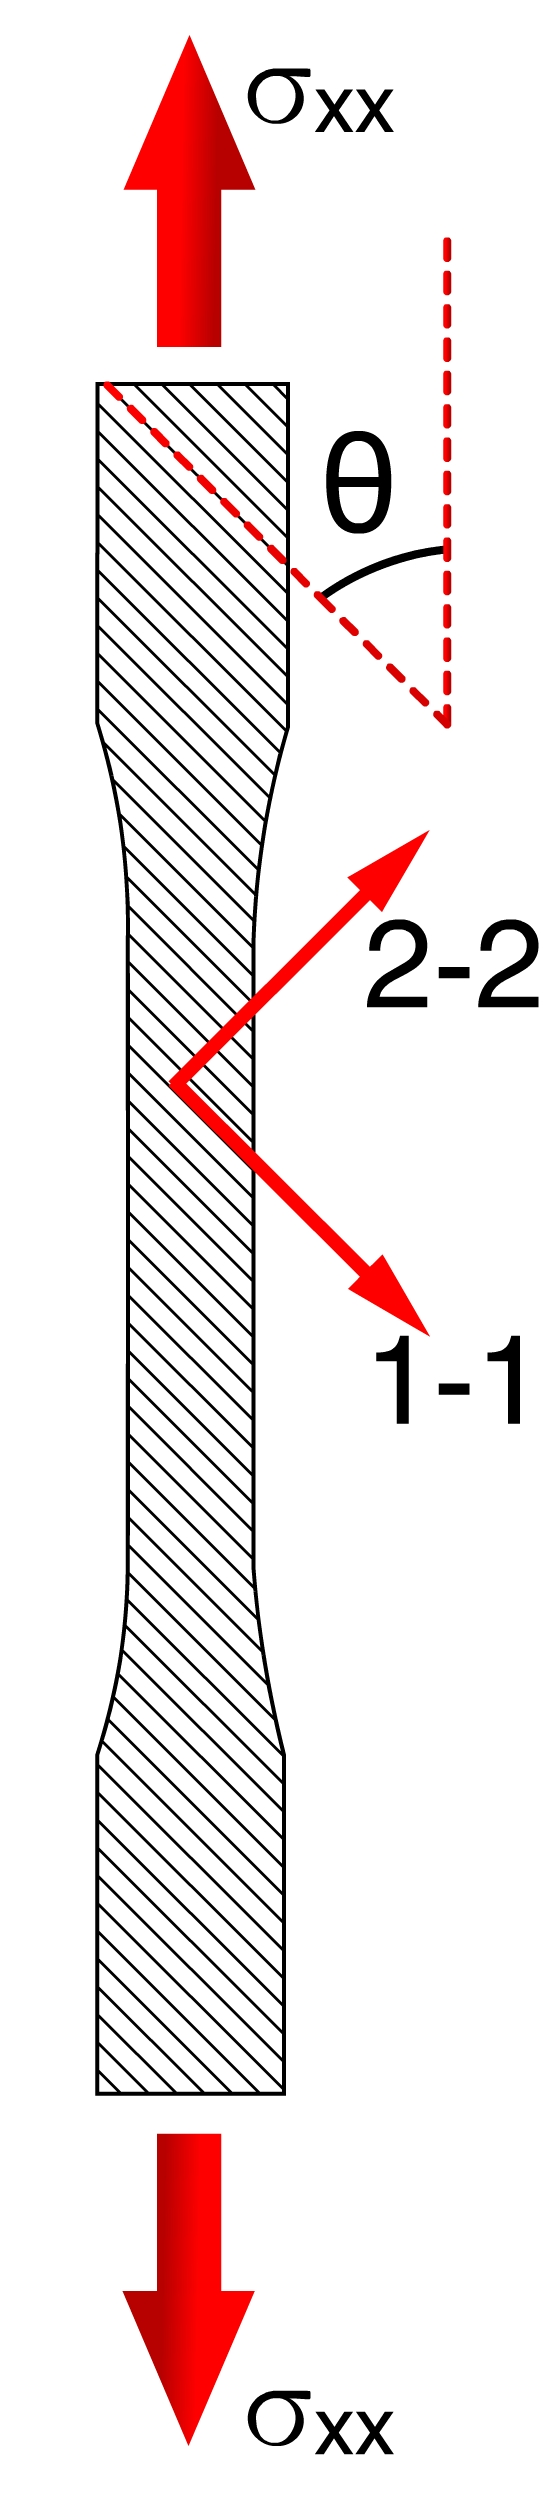
\includegraphics[height=9.5cm, keepaspectratio]{compl_load.jpg}
	\caption{Off-axis loading conditions}
	\label{fig:offaxis}
\end{figure}

Using this type of loading condition, the results can be converted to the principal coordinate system by using the following transformation:

\begin{equation} \label{eq:comp_matrix}
	\left\{\begin{matrix}\sigma_{11}\\\sigma_{22}\\\tau_{12}\\\end{matrix}\right\}=\left[\begin{matrix}\cos^2{\theta}&\sin^2{\theta}&2.\cos{\theta.\sin{\theta}}\\\sin^2{\theta}&\cos^2{\theta}&-2.\cos{\theta.\sin{\theta}}\\-\cos{\theta.\sin{\theta}}&\cos{\theta.\sin{\theta}}&\cos^2{\theta-\sin^2{\theta}}\\\end{matrix}\right]\left\{\begin{matrix}\sigma_{xx}\\0\\0\\\end{matrix}\right\}
\end{equation}

This study proposes verification of the previously developed envelope through this type of uniaxial test. Multiple FFF coupons produced with a variety of raster angles are used to compare the resulting complex stress states in the local coordinate system of the part, to the failure line determined through application of the failure criterion.

\section{Experimental Methods} \label{sec:exmet_ssic}

The toolpath of tensile coupons was generated using the SciSlice engine \cite{VanHulle2017a}, following the ASTM D-638 Type I standard geometry \cite{ASTMD638} due to a lack of a standardized test for AM parts. In order to test a variety of combined loading scenarios, six raster configurations were selected: 0°, 30°, 45°, 60°, 75°, and 90° with respect to the loading direction, as depicted in Figure \ref{fig:offaxis}. Each orientation was replicated five times. The printing conditions were exactly the same as those used by the authors to generate the original failure envelope. These are shown in Table \ref{tab:printparam_ssic}. Specimens were printed in a traditional desktop 3D printer (Lulzbot TAZ5, USA), using a customized 2.85 mm ABS filament extruded in-house, based on the Cycolac MG94 material produced by SABIC.

\begin{table}[!htbp] 
	\renewcommand{\arraystretch}{1.5}
	\centering
	\caption{Printing parameters maintained constant.}
	\newcolumntype{C}{ >{\centering\arraybackslash} m{0.25\linewidth} }
	\newcolumntype{M}{ >{\centering\arraybackslash} m{0.15\linewidth} }
	\begin{tabular}{C C} 
		\toprule
		\textbf{Printing Parameter} & \textbf{Value}\\
		\midrule
		Nozzle Temperature & $220\ ^\circ C$ \\
		Bed Temperature & $100\ ^\circ C$\\
		Printing Speed & $2000 \  mm/min$\\
		Layer Height & $0.2\  mm$\\
		Path Width & $0.4\  mm$\\
		Extrusion Factor & $1$\\
		\bottomrule
	\end{tabular}
	\label{tab:printparam_ssic}
\end{table}

Mechanical tests were conducted on an Instron 5967 dual column universal testing machine with a 30 kN load cell, using the recommended testing speed of $5\ mm/min$, dictated by the ASTM standard \cite{ASTMD638}. All of the data acquisition was handled through the accompanying Instron Bluehill 3 software. The resulting experimental data was compared to the original failure envelope developed by the authors in previous work. To better visualize the results, the original mathematical formula, expressed in terms of stresses in the local coordinate system of the polymer beads, was translated into the global coordinate system. The transformation involves using the relation shown in Equation \ref{eq:comp_matrix}, resulting in the following system of equations. Solving for $\sigma_{xx}$ allows the failure surface to be expressed as a function of the raster angle and the tensorial components. 

\begin{equation}
	\sigma_{11}=\sigma_{xx}.{\cos{\left(\theta\right)}}^2;\ \ \sigma_{22}=\sigma_{xx}.{\sin{\left(\theta\right)}}^2;\ \tau_{12}=-\sigma_{xx}.\cos{\theta.\sin{\theta}}
\end{equation}

\begin{equation}
	\begin{split}
		1=F_{11}\sigma_{11}+F_{22}\sigma_{22}+F_{12}\tau_{12}\\ +\left(F_{1111}\sigma_{11}^2+F_{2222}\sigma_{22}^2+F_{1212}\tau_{12}^2+2F_{1122}\sigma_{11}\sigma_{22}+2F_{1112}\sigma_{11}\tau_{12}+2F_{2212}\sigma_{22}\tau_{12}\right)^{1/2}
	\end{split}
\end{equation}

\end{document}